\documentclass[11pt,letterpaper]{article}
\usepackage[T1]{fontenc}
\usepackage{lmodern,amsmath,amssymb,amsthm,mathtools,microtype,booktabs}
\usepackage[letterpaper,left=1.05in,right=1.05in,top=.9in,bottom=.94in,headheight=14pt,headsep=.25in]{geometry}
\usepackage{fancyhdr,xcolor}
\definecolor{ink}{HTML}{183C51}
\definecolor{accent}{HTML}{12655F}
\usepackage[colorlinks=true,linkcolor=accent,citecolor=accent,urlcolor=accent,pdftitle={Which samples of Li coefficients detect off-line zeros?}]{hyperref}
\usepackage{enumitem,graphicx,needspace}
\setlist{nosep,leftmargin=*}
\pagestyle{fancy}\fancyhf{}\lhead{\small\textcolor{ink}{Sampling Li coefficients}}\rhead{\small\textcolor{ink}{November 2026}}\cfoot{\thepage}
\renewcommand{\headrulewidth}{.25pt}
\newtheorem{theorem}{Theorem}
\newtheorem{lemma}[theorem]{Lemma}
\newtheorem{corollary}[theorem]{Corollary}
\newtheorem{proposition}[theorem]{Proposition}
\newcommand{\T}{\mathbb T}
\newcommand{\Z}{\mathbb Z}
\newcommand{\N}{\mathbb N}
\newcommand{\C}{\mathbb C}
\newcommand{\R}{\mathbb R}
\newcommand{\Rea}{\operatorname{Re}}
\newcommand{\Ima}{\operatorname{Im}}
\newcommand{\dist}[1]{\lVert #1\rVert_{\T}}
\newcommand{\dc}{\underline d_{\mathrm B}}
\newcommand{\smalltitle}[1]{\par\medskip\noindent{\color{ink}\textbf{#1}}\enspace}
\setlength{\emergencystretch}{1.8em}
\raggedbottom
\begin{document}
\thispagestyle{plain}
{\small\sffamily\bfseries\color{accent} ANALYTIC NUMBER THEORY \hfill 26 NOVEMBER 2026}
\par\vspace{1.15em}
{\huge\bfseries\color{ink} Which samples of Li coefficients\\[2pt] detect off-line zeros?\par}
\vspace{.65em}
{\large Joint tests at polynomial indices and sign patterns for Riemann's \(\xi\)\par}
\vspace{.85em}\noindent\rule{\textwidth}{.7pt}
\begin{abstract}\noindent
We characterize the schedules on which every symmetric strip spectrum with an off-line zero has simultaneously negative Li coefficients. The exact condition is recurrence to the identity in every finite torus. A missed neighborhood yields a real polynomial whose zeros lie in the strip and whose Li coefficients defeat the proposed test. For polynomial schedules the criterion is a common root modulo every integer. When the parameter is prime, the root must be a unit. For the Riemann zeta function itself, let \(d_n\) be the centered second difference of its Li coefficients. Each of the four sign pairs of \((d_k,d_{k^2})\) occurs on a set of positive lower Banach density with both magnitudes greater than \(0.011\). The first negative second difference is \(d_{118}\). The initial signs imply maximal runs of exactly 235 positive second differences recurring simultaneously around \(k^2\) and \(k^3\), with a negative value immediately before and after each run. The sign thresholds follow from rigorous interval estimates and the recurrence theorem.
\end{abstract}
\section{The sampling question}
Write \(u_\rho=1-1/\rho\). The critical line \(\Rea\rho=1/2\) maps to \(|u_\rho|=1\).
Li's coefficients sum the real parts of \(1-u_\rho^n\) over zeros. On the line every summand is nonnegative. An off-line zero introduces exponentially large oscillations. Which indices guarantee seeing the negative sign? If several measurements are made at once, when must all of them be negative?
\par\smallskip
For any symmetric spectrum as in \eqref{eq:spectrum} that has an off-line zero, \(L_{k^2}\) and \(L_{k^3}\) are both negative for a positive lower density of \(k\). The indices \((p-1)^2,p^2-1\) have the same property for a positive fraction of primes. The pair \(k,k+1\) behaves differently. Each coordinate separately detects every defect, yet a polynomial of degree two defeats simultaneous detection at every \(k\).
\par\smallskip
For actual Riemann zeros the unit-circle geometry instead gives a positive measure of finite mass. Its Fourier coefficients are the second differences \(d_n\). This turns sufficiently accurate measurements at a handful of indices into conclusions about infinitely many sign patterns. The proofs of the sampling criterion and of its arithmetic application use the two sides of this same geometry.

\section{Spectra and dominant terms}
A \emph{symmetric strip spectrum} is a locally finite multiset \(\mathcal Z\) in the open critical strip, with finite multiplicities, invariant under conjugation and \(\rho\mapsto1-\rho\), such that
\begin{equation}
 0<\Rea\rho<1,\qquad W=\sum_{\rho\in\mathcal Z} |\rho|^{-2}<\infty .
 \label{eq:spectrum}
\end{equation}
Sums over zeros count multiplicity. Write \(\N=\{1,2,\ldots\}\). Define
\begin{equation}
 L_0=0,\qquad L_n=\sum_{\rho\in\mathcal Z}\bigl(1-\Rea u_\rho^n\bigr)\quad(n\ge1),
 \qquad L_{-n}=L_n . \label{eq:li}
\end{equation}
For Riemann's \(\xi\), these are the classical real Li coefficients. For a nonreal primitive Dirichlet character the union of the nontrivial zero multisets of \(L(s,\chi)\) and \(L(s,\bar\chi)\) has both symmetries. The usual \(O(T\log(T+2))\) zero count for a fixed completed zeta or Dirichlet \(L\)-function gives \eqref{eq:spectrum} by partial summation \cite{lag}.
\begin{lemma}[Dominant phases]\label{lem:dom}
On the critical line \(L_n\ge0\). In every other case there is a largest radius \(R>1\) of the \(u_\rho\). List the arguments on this circle, with multiplicity, as \(2\pi\alpha_1,\ldots,2\pi\alpha_m\). There is \(1<r<R\) for which
\[
 R^{-n}L_n=-\sum_{j=1}^m\cos(2\pi n\alpha_j)
         +O_{\mathcal Z}\bigl(n^2(r/R)^n\bigr).
\]
\end{lemma}
\begin{proof}
The identity \(|u_\rho|^2=1+(1-2\Rea\rho)/|\rho|^2\) and reflection give an outer point. Only finitely many \(u_\rho\) lie outside any fixed neighborhood of \(1\), by \eqref{eq:spectrum}. This gives a finite dominant circle and a strict gap to the remaining radii. For the remaining points the segment from \(1\) to \(u_\rho\) lies in \(|z|\le r\). Taylor's integral remainder gives
\[
 \bigl|u_\rho^n-1+n/\rho\bigr|\le \tfrac12 n(n-1)r^{n-2}|\rho|^{-2}\quad(n\ge2).
\]
Also \(0<\Rea(1/\rho)<|\rho|^{-2}\). Thus \eqref{eq:li} converges absolutely in the real-part convention. Summation on the complement gives the stated error. On the line each summand in \eqref{eq:li} is nonnegative.
\end{proof}
\smalltitle{Schedules.}
Fix \(s\ge1\) and positive indices \(n_1(k),\ldots,n_s(k)\), with \(\min_i n_i(k)\to\infty\). Dropping finitely many parameters gives the same eventual test. Write \(\T=\R/\Z\), \(\dist{x}=\min_{j\in\Z}|x-j|\). The schedule has \emph{simultaneous Bohr recurrence} if for every \(d\ge1\), \(\alpha\in\T^d\), and \(\delta>0\), there are arbitrarily large \(k\) such that
\begin{equation}
 \max_{i\le s,\,j\le d}\dist{n_i(k)\alpha_j}<\delta . \label{eq:return}
\end{equation}

\section{An exact criterion for arbitrary schedules}
\begin{theorem}[Universal Li sampling]\label{thm:general}
For any schedule as above the following conditions are equivalent.
\begin{enumerate}[label=\textup{(\roman*)}]
\item The schedule has simultaneous Bohr recurrence.
\item For every symmetric strip spectrum with an off-line zero,
\(\max_i L_{n_i(k)}<0\) for arbitrarily large \(k\).
\item For every such spectrum, with \(R,m\) as in Lemma~\ref{lem:dom},
\[
 \liminf_{k\to\infty}\ \max_{1\le i\le s} R^{-n_i(k)} L_{n_i(k)}=-m .
\]
\end{enumerate}
When \textup{(i)} fails there is a single finite off-line spectrum for which at least one sampled coefficient is strictly positive at \emph{every} parameter. Its zeros may be arbitrarily close to the critical line.
\end{theorem}
\begin{proof}
Apply \eqref{eq:return} to the dominant phases in Lemma~\ref{lem:dom} with tolerances tending to zero. All the cosines approach one at every coordinate of the schedule. Their sum is at most \(m\), giving (iii). Since \(m\ge1\), (iii) implies (ii).

Suppose (i) fails. Choose phases \(\alpha_1,\ldots,\alpha_d\) and \(0<\delta<1/2\) for which \eqref{eq:return} eventually fails. If necessary append one irrational phase and shrink \(\delta\) to exclude the finitely many exceptional parameters: all their indices are positive, so none of their multiples of that phase is zero. For every \(k\) some \(n=n_i(k)\) now has \(n\alpha\) outside the open \(\delta\)-cube about zero.
Consider
\[
 K_b(x)=\prod_{j=1}^{d}\left(\frac{1+\cos(2\pi x_j)}2\right)^b
       =\sum_h a_h\,e^{2\pi i h\cdot x}\qquad (b\in\N).
\]
All \(a_h\) are nonnegative dyadic rationals and \(a_{-h}=a_h\).
In one coordinate the constant coefficient \(4^{-b}\binom{2b}{b}\) is the largest by the binomial theorem. There are \(2b+1\) coefficients with total mass one. Hence \(a_0\ge(2b+1)^{-d}\).
Outside the cube \(K_b(x)\le\cos^{2b}(\pi\delta)\).
Choose \(b\) so this is strictly below \(a_0\).
Put \(c=\sum_{h:\,h\cdot\alpha\in\Z}a_h\ge a_0\). Clearing a common denominator \(D_0\) and collecting equal phases gives
\[
 T(n)=D_0\bigl(K_b(n\alpha)-c\bigr)
     =\sum_{v\in V} b_v v^n,\qquad |v|=1,\quad v\ne1,\quad b_v=b_{\bar v}\in\N .
\]
The finite set \(V\) is nonempty, since \(T(n)<0\) at every missed index just described.

Take Cayley points \(Rv,R^{-1}v\), each with multiplicity \(b_v\), where \(R>1\) is sufficiently close to one. At \(R=1\) each inverse image \(1/(1-v)\) has real part \(1/2\). Continuity and finiteness put all the perturbed inverse images inside the strip, as close to the line as desired. Conjugation and inversion preserve the Cayley multiset, hence both zero symmetries hold. If \(B=\sum_v b_v\), direct substitution yields
\begin{equation}
 L_n=2B-(R^n+R^{-n})T(n) . \label{eq:counter}
\end{equation}
At each \(k\) at least one such value exceeds \(2B\). This contradicts (ii).
\end{proof}

\begin{corollary}[Finite perturbations of Riemann's \(\xi\)]\label{cor:xi}
In the failure case a counterexample can also be an entire function of order one, real on the real axis and invariant under \(z\mapsto1-z\). Its zeros agree with those of \(\xi\), with multiplicities, above some finite absolute height. Its total number of zeros in \(|\Ima z|\le T\) agrees exactly with that of \(\xi\) for every sufficiently large \(T\).
\end{corollary}
\begin{proof}
Let \(A\) be the monic polynomial with the \(2B\) zeros in \eqref{eq:counter}. Choose \(B\) conjugate pairs of nonreal zeros of \(\xi\) on the critical line, respecting their multiplicities, and form their monic polynomial \(H\). Both polynomials are real, monic of degree \(2B\), and even about \(1/2\). The function \(F=\xi A/H\) is entire with the stated symmetry and zero counts. At infinity \(A/H=1+O(|z|^{-2})\), since the leading terms and sums of roots agree, so the order is preserved. The retained zeros of \(\xi\) lie on the line by RH and give nonnegative contributions at every index. The strict positive witness survives. The construction uses the functional equation and the zeros; an Euler product would be an additional arithmetic constraint.
\end{proof}
\section{Polynomial indices over integers and primes}
For \(E\subset\N\), its lower Banach density is
\[
 \dc(E)=\liminf_{H\to\infty}\inf_{a\in\Z_{\ge0}}
       \frac{\#(E\cap(a,a+H])}{H}.
\]
For primes use lower relative density
\(\liminf_{X\to\infty}\#\{p\in E:p\le X\}/\pi(X)\).
These measure the abundance of successful parameters. A set of sampled coefficient indices such as the squares can itself have density zero.
\Needspace{9\baselineskip}
\begin{theorem}[The common-root criterion]\label{thm:poly}
Let \(P_1,\ldots,P_s\in\Z[x]\) be nonconstant with positive leading coefficients. Ignore parameters at which some index is nonpositive.
\begin{enumerate}[label=\textup{(\alph*)}]
\item Over integers \(k\ge1\), the universal tests of Theorem~\ref{thm:general} hold for \(n_i(k)=P_i(k)\) if and only if every modulus \(q\ge1\) admits a common root of the \(P_i\).
\item Over primes \(p\), the tests hold if and only if every modulus admits a common root coprime to \(q\).
\end{enumerate}
Under the corresponding condition, for every off-line spectrum and \(0<\eta<1\), the set where
\[
 \max_i R^{-P_i(k)} L_{P_i(k)}<-(1-\eta)m
\]
has positive lower Banach density in \textup{(a)} and positive lower relative prime density in \textup{(b)}. One set of good parameters works for any finite family of off-line spectra, using its own \(R,m\) for each.
\end{theorem}
\begin{proof}
For necessity take the phase \(1/q\) in \eqref{eq:return} with tolerance \(1/(2q)\). A prime larger than \(q\) is a unit modulo \(q\). Theorem~\ref{thm:general} supplies a strip counterexample if the test fails.

For sufficiency, fix \(\alpha\in\T^d\). Choose real representatives and a rational basis \(1,\beta_1,\ldots,\beta_t\) for their rational span together with \(1\). Write \(D\alpha_j=b_j+\sum_\ell a_{j\ell}\beta_\ell\), with all coefficients integral and \(D\ge1\). Choose a common root \(u\bmod D\), a unit in the prime case. In that class consider
\(X(k)=(P_i(k)\alpha_j)_{ij}\). For a character \(h=(h_{ij})\in\Z^{sd}\), put
\[
 C_\ell(x)=\sum_{i,j}h_{ij}a_{j\ell}P_i(x).
\]
If \(C_\ell\) is constant, evaluating at a common root modulo each \(q\) shows that constant is zero. Set
\(\Lambda=\{h:C_\ell\equiv0\ \text{for all }\ell\}\), and
\(H=\{x\in\T^{sd}:h\cdot x=0\bmod1\ \text{for all }h\in\Lambda\}\).
On \(k\equiv u\bmod D\) the rational term
\(D^{-1}\sum h_{ij}b_jP_i(k)\) is integral. If \(h\notin\Lambda\), the polynomial \(D^{-1}\sum_\ell \beta_\ell C_\ell(x)\) has an irrational leading coefficient in positive degree, by rational independence.
Along \(k=u+Dt'\) the corresponding character has mean zero by Weyl's theorem \cite{weyl}. This convergence is uniform over the starting integer of a long interval in \(t'\). In degree one the geometric sum is bounded uniformly. Induction by the van der Corput difference inequality applies in higher degree: for each fixed nonzero step the difference has irrational leading coefficient independent of the starting point. Taking the interval length to infinity first, then the number of differences to infinity, gives uniform convergence.

For primes in the same reduced class, expand the indicator of \(p\equiv u\bmod D\) as a sum of additive characters in \(p\). Each added term \(ap/D\) preserves irrationality of a nonconstant coefficient. Rhin's polynomial equidistribution theorem \cite{rhin} gives mean zero over primes for each resulting exponential. The prime number theorem in fixed arithmetic progressions gives relative mass \(1/\varphi(D)\) for the class. Characters in \(\Lambda\) are identically one in that class.

In both settings the limiting probability measure on the progression is Haar probability on \(H\). Indeed, its Fourier transform is one on \(\Lambda\) and zero off \(\Lambda\), by the annihilator identity for subgroups of \(\Z^{sd}\). Approximation by trigonometric polynomials gives convergence for continuous functions, uniform over starting points in the integer case. The argument includes \(t=0\), when all phases are rational.

Every relative neighborhood of zero in \(H\) has positive measure. Test against a continuous nonnegative function supported in the chosen cube and positive at zero. This gives positive lower density of returns on the progression, and hence in the full parameter set. Concatenate all dominant angles for the last assertion and apply Lemma~\ref{lem:dom}.
\end{proof}

\section{Examples and explicit obstructions}
\begin{center}\small
\begin{tabular}{@{}lll@{}}
\toprule
Indices at parameter \(x\) & Integer parameters & Prime parameters\\
\midrule
\(x^2,\ x^3\) & Detect & Fail modulo \(2\) eventually\\
\((x-1)^2,\ x^2-1\) & Detect & Detect\\
\(x,\ x+1\) & Fail modulo \(2\) & Fail modulo \(2\)\\
\(J(x),\ (x+2)J(x)\) below & Detect & Detect\\
\bottomrule
\end{tabular}
\end{center}
Detection means simultaneous negative values for every admissible off-line spectrum. A prime can use the residue class \(0\bmod 2\) only once.
\smalltitle{A polynomial with no integer root.}
Let \(J(x)=(x^2-13)(x^2-17)(x^2-221)\).
At an odd prime \(\ell\nmid221\), one of \(13,17,221\) is a nonzero square modulo \(\ell\): if the first two are nonsquares their product is a square. A root of the relevant quadratic is simple and lifts to every power of \(\ell\). At \(13\) use \(17\equiv4\), and at \(17\) use \(13\equiv 8^2\). At \(2\) use \(17\equiv1\bmod8\), so \(17\) is a square in \(\Z_2^\times\). These roots are units. The Chinese remainder theorem supplies a unit root modulo every \(q\), although none of the three constants is a square integer.
\smalltitle{A rational polynomial for a failed modulus.}
For \(q\ge2\), take both radii \(R,R^{-1}\) above all nonidentity \(q\)-th roots of unity, with \(R>1\) rational sufficiently close to one. The phase sum is \(q-1\) at a multiple of \(q\) and \(-1\) elsewhere, giving
\begin{equation}
 L_n=
 \begin{cases}
   (q-1)(2-R^n-R^{-n})<0,&q\mid n,\\[2pt]
   2(q-1)+R^n+R^{-n}>0,&q\nmid n .
 \end{cases} \label{eq:cyclo}
\end{equation}
The zeros are roots of a rational-coefficient polynomial proportional to
\[
 \prod_{t\in\{R,R^{-1}\}}
 \frac{(z-1)^q-t^q z^q}{(z-1)-tz}.
\]
For \(q=2,R=2\) take \(9z^2-9z+2\). Its zeros are \(1/3,2/3\), its Cayley points are \(-2,-1/2\), and its Li coefficients are negative precisely at positive even indices. No two consecutive coefficients are both negative.
\smalltitle{An obstruction invisible to divisibility.}
Put \(v=(3+4i)/5=e^{2\pi i\theta}\). It has infinite order since \(v+\bar v=6/5\) is rational and fails to be an algebraic integer. The set \(S=\{n:\Rea(v^n)\le-1/2\}\) meets every \(q\N\) infinitely often by irrational rotation. Yet \(R^{\pm1}v,R^{\pm1}\bar v\) with \(R=6/5\) give \(L_n=4-2(R^n+R^{-n})\Rea(v^n)>0\) on \(S\). The four zeros form the rectangle
\(\{7/25,18/25\}+\{24i/25,-24i/25\}\).
Thus the congruence criterion for polynomial schedules would be false for arbitrary sets of indices.

\Needspace{11\baselineskip}
\section{A measurement that controls every shift}
For a nonempty symmetric on-line spectrum write
\[
 d_n=L_{n+1}-2L_n+L_{n-1},\qquad C=d_0=2L_1,\qquad n\in\Z .
\]
\begin{theorem}[Uniform recurrence of Li second differences]\label{thm:curv}
For every \(h\in\Z\),
\begin{equation}
 C-d_h\ \le\ \sup_{n\in\Z}|d_{n+h}-d_n|
 \ \le\ \sqrt{2C(C-d_h)} . \label{eq:cert}
\end{equation}
The upper bound is sharp on symmetric on-line spectra. For polynomial schedules satisfying Theorem~\ref{thm:poly}\textup{(a)} or \textup{(b)}, and any \(\epsilon>0\),
\[
 \max_i\sup_{n\in\Z}|d_{n+P_i(k)}-d_n|<\epsilon
\]
on a set of positive lower Banach or lower relative prime density, respectively. The same parameters work for any prescribed finite family of such spectra. In particular \(\limsup_k\min_i d_{P_i(k)}=C\).
\end{theorem}
\begin{proof}
Set \(a_\rho=|1-u_\rho|^2=|\rho|^{-2}\). Centered second differences in \eqref{eq:li} give the absolutely and uniformly convergent Fourier series
\begin{equation}
 d_n=\sum_\rho a_\rho u_\rho^n,\qquad C=\sum_\rho a_\rho. \label{eq:fourier}
\end{equation}
Conjugation makes this real. Taking \(n=0\) in the supremum gives the lower bound. For the upper bound apply Cauchy--Schwarz to \(\sum a_\rho|u_\rho^h-1|\), using \(\sum a_\rho|u_\rho^h-1|^2=2(C-d_h)\). A conjugate pair \(u_\rho=e^{\pm2\pi i\theta}\) with \(\theta\) irrational has \(d_n=C\cos(2\pi n\theta)\). Density of irrational rotations gives a supremum of \(2C|\sin(\pi h\theta)|\), which attains the bound. For recurrence truncate \eqref{eq:fourier} to leave omitted mass below \(\epsilon/4\). Simultaneous returns make \(\sum_{\mathrm{retained}}a_\rho|u_\rho^{P_i(k)}-1|<\epsilon/2\) for every \(i\). The tail costs at most twice its mass, uniformly in \(n\). Apply the density argument in Theorem~\ref{thm:poly} to the retained phases. Use their union for finitely many spectra.
\end{proof}
Dirichlet GRH makes this conclusion applicable to the paired primitive characters described after \eqref{eq:li}, or to a single real primitive character. For \(\xi\), the ceiling \(C=2+\gamma-\log(4\pi)\) is approached arbitrarily closely. For each nonzero \(h\) one has \(d_h<C\), since equality would require every Cayley point to be an \(h\)-th root of unity, whereas \(\xi\) has infinitely many distinct zeros.
\section{Four signs for the pair \texorpdfstring{\((d_n,d_{n^2})\)}{of second differences}}
\label{sec:signs}

Write $d_n=\lambda_{n+1}-2\lambda_n+\lambda_{n-1}$ for the centered
second difference of the classical Riemann Li coefficients.
The simultaneous signs of $d_n$ and $d_{n^2}$ describe the local convexity
or concavity of the same sequence at two widely separated indices.

\begin{corollary}\label{cor:signs}
For each $(a,b)\in\{-1,1\}^2$, the set
\[
 \{n\ge1:\ ad_n>11/1000,\quad bd_{n^2}>11/1000\}
\]
has positive lower Banach density. For the corresponding $h$ in
Table~\ref{tab:seeds}, these inequalities also hold at $n=h+p-1$
for a set of primes $p$ of positive lower density relative to the primes.
The same set of primes can be used for all four rows.
\end{corollary}

\begin{table}[ht]
\centering
\begin{tabular}{rcc@{\qquad}rr}
\hline
$h$ & $a$ & $b$ & lower bound for $ad_h$ & lower bound for $bd_{h^2}$\\
\hline
891327 & $+$ & $+$ & 0.01161 & 0.01387\\
842728 & $+$ & $-$ & 0.01180 & 0.01349\\
602346 & $-$ & $+$ & 0.01165 & 0.01133\\
673696 & $-$ & $-$ & 0.01119 & 0.01148\\
\hline
\end{tabular}
\caption{Certified strict inequalities for the Riemann zeta function.
Every decimal in the two right columns denotes an exact rational number.}
\label{tab:seeds}
\end{table}

\begin{proof}
First take the inequalities in the table, verified below. The polynomials
$u$ and $2hu+u^2$ vanish at $u=0$. The simultaneous uniform returns from
Theorem~\ref{thm:curv} therefore give a set of $u$ of positive lower
Banach density for which both $d_{h+u}$ and $d_{h^2+2hu+u^2}$ are arbitrarily
close to their respective values at $h$ and $h^2$. Take the tolerance
smaller than the least margin in the chosen row and put $n=h+u$.
For the prime assertion, the polynomials $p-1$ and
$(p-1)(2h+p-1)$ have the common unit root $1$ modulo every positive
integer. Take the finite family consisting of $p-1$ and all four
polynomials $(p-1)(2h+p-1)$. Their common unit root $1$ gives
simultaneous returns with $u=p-1$ for every row.
\end{proof}

\paragraph{Verification of Table~\ref{tab:seeds}.}
We use forty conjugate pairs of zeros. Their contribution can be certified
without resolving every zero below a height. Under RH a pair with positive
ordinate $t$ contributes $w(t)\cos(n\theta(t))$ to $d_n$, where
\[
 w(t)=\frac{2}{1/4+t^2},\qquad
 \theta(t)=2\arctan\!\frac{1}{2t}.
\]
The total mass of all pairs is $C=2+\gamma-\log(4\pi)$, as in
Theorem~\ref{thm:curv}. If $t_1,\ldots,t_{40}$ are the certified
ordinates, put $W=C-\sum_j w(t_j)$. For either $e\in\{-1,1\}$,
\begin{equation}
 ed_n\ \ge\ \sum_{j=1}^{40}e\,w(t_j)\cos\bigl(n\theta(t_j)\bigr)-W.
 \label{eq:signedtail}
\end{equation}
Here $0.01022325<W<0.01022326$.

The verifier starts with forty decimal centers $s_0=1/2+it_0$,
$13<t_0<130$. It assigns each the disk of radius $r=10^{-18}$ and
checks that the ordinate intervals are disjoint. At both $s=s_0$ and
$s=s_0+10^{-6}$ it evaluates $\zeta(s)$ by Euler--Maclaurin summation,
with cutoff $N=256$ and $m=20$ Bernoulli corrections. The explicit formula is
\[
 \sum_{j=1}^{N-1} j^{-s} + \frac{N^{1-s}}{s-1} + \frac{N^{-s}}{2}
 + \sum_{k=1}^{m}\frac{B_{2k}}{(2k)!}(s)_{2k-1}N^{1-s-2k} + R.
\]
Here $(s)_j$ is a rising factorial. The Fourier series for the periodic
Bernoulli polynomial gives
\[
 |R|\le \frac{2\zeta(2m)}{(2\pi)^{2m}}\,
 |(s)_{2m}|\frac{N^{1-\Re s-2m}}{\Re s+2m-1}
 \le 4N\left(\frac{171}{6N}\right)^{40}<10^{-34}.
\]
The code generates the Bernoulli numbers over the rationals and performs
all transcendental evaluations with outward-rounded 192-bit MPFI intervals.

For every center, the calculation gives $|\zeta(s_0)|<2\cdot10^{-25}$
and a coordinate of the difference quotient with absolute value greater
than $0.1$. To turn this into a zero certificate, first-order Euler
summation on $|s-s_0|\le1/4$ gives
$|\zeta(s)|\le |s-1|^{-1}+1/2+|s|/(2\Re s)<300$.
By Cauchy's estimate the Taylor terms of degree at least two sum in
absolute value to at most
$300(4|v|)^2/(1-4|v|)<5000|v|^2$ for $0<|v|\le10^{-6}$.
Thus $|\zeta'(s_0)|>0.1-5000\cdot10^{-6}>0.09$.
On $|v|=r$ the linear term exceeds in modulus the sum of the constant
term and the Taylor remainder. Rouch\'e's theorem gives one zero
counted with multiplicity inside each disk. Inserting each entire
ordinate interval into \eqref{eq:signedtail} yields
Table~\ref{tab:seeds}. All seeds, enclosures, and comparisons can be
reproduced by running \texttt{certify\_zeta.py}.

\section{Convexity intervals from two Li coefficients}
\label{sec:windows}

Let $\lambda_n$ be the Li coefficients of the completed Riemann zeta
function, with $\lambda_0=0$ and $\lambda_{-n}=\lambda_n$. Write
\[
 d_n=\lambda_{n+1}-2\lambda_n+\lambda_{n-1},\qquad
 C=d_0=2\lambda_1,\qquad \tau=C-d_1=4\lambda_1-\lambda_2 .
\]
The critical-line theorem gives a concrete pattern in this sequence.
A set of integers $k$ of positive lower Banach density satisfies
\begin{align}
 d_{k^2+j},\ d_{k^3+j}&>0.00034 && (|j|\le39),\label{eq:79window}\\
 d_{k^2+j},\ d_{k^3+j}&>0.00070 && (|j|\le35).\label{eq:71window}
\end{align}
Thus 79 consecutive strictly positive second differences recur
simultaneously around a square and a cube. Both bounds use only the
first two Li coefficients to establish the starting interval. The
recurrence then uses the full spectrum. Every finite jointly
intersective family tending to $+\infty$ can replace the square and
cube in these conclusions by Theorem~\ref{thm:curv}. The prime-index version applies, for instance, to \((p-1)^2,p^2-1\).

\paragraph{A bound from two moments.}
For a nontrivial zero $\rho$, let $u_\rho=1-1/\rho$,
$w_\rho=|1-u_\rho|^2$ and $x_\rho=\operatorname{Re}u_\rho$.
Under RH, $|u_\rho|=1$. The Fourier series for $d_n$ gives a
probability measure $\mu=C^{-1}\sum_\rho w_\rho\delta_{x_\rho}$ on
$[-1,1]$. If $T_j(\cos\theta)=\cos(j\theta)$ is the Chebyshev
polynomial, then
\[
 \frac{d_j}{C}=\int T_{|j|}(x)\,d\mu(x),\qquad
 a=\int x\,d\mu(x)=\frac{d_1}{C}=1-\frac{\tau}{C}.
\]
For $j\ge2$ put $b_j=\cos(\pi/j)$. The function equal to $-1$ on
$[-1,b_j]$ and to $T_j$ on $[b_j,1]$ is a convex minorant of $T_j$.
Indeed, for $0<\theta<\pi/j$,
\[
 T'_j(\cos\theta)
   =j\,\frac{\sin(j\theta)}{\sin\theta}
   =j\sum_{r=0}^{j-1}\cos\big((j-1-2r)\theta\big).
\]
Each summand is nonincreasing in $\theta$, since its argument in
absolute value lies in $[0,\pi)$. Thus $T'_j$ is nondecreasing on
$[b_j,1]$ and its value at $b_j$ is zero. Jensen's inequality gives
\[
 a\ge b_j\quad\Longrightarrow\quad d_j\ge C T_j(a).
\]
For the normalized problem with the first moment $a$ prescribed, this
bound on $[b_j,1]$ is attained by $\mu=\delta_a$. For
$-1<a<1$ the corresponding normalized sequence is realized by one
conjugate pair of critical-line zeros with Cayley phases
$\pm\arccos(a)$.

An estimate with a larger margin on a shorter interval follows from
$|1-u^j|\le |j|\,|1-u|$ for $|u|=1$. Summing gives
\[
 C-d_j=\tfrac12\sum_\rho w_\rho |1-u_\rho^j|^2
       \le j^2\tau .
\]

\paragraph{Exact arithmetic for the bounds.}
Use $\gamma$ for Euler's constant and the sign convention
$\zeta(1+x)=x^{-1}+\gamma-\gamma_1 x+O(x^2)$. Put
$L(s)=\log\xi(s)$ near $s=1$. Li's derivative formula gives
$\lambda_1=L'(1)$ and $\lambda_2=2L'(1)+L''(1)$. In the logarithm
of $\xi(s)=s(s-1)\pi^{-s/2}\Gamma(s/2)\zeta(s)/2$, expand
$(s-1)\zeta(s)$ at $s=1$ and use
$\psi(1/2)=-\gamma-2\log 2$ and $\psi'(1/2)=\pi^2/2$. This yields
\[
 \lambda_1=1+\frac{\gamma-\log(4\pi)}{2},\qquad
 \lambda_2=2\lambda_1-1+\frac{\pi^2}{8}-\gamma^2-2\gamma_1.
\]
The accompanying \texttt{constants\_verify.py} certifies
\begin{align*}
 0.0007430 &< C-35^2\tau < 0.0007433,\\
 0.0003500 &< C T_{39}(a) < 0.0003504,\\
 -0.0015012 &< C T_{40}(a) < -0.0015008 .
\end{align*}
It verifies $a>1-2/40^2\ge\cos(\pi/40)$, where the latter inequality
comes from $\sin t\ge2t/\pi$ on $[0,\pi/2]$. Consequently
$0\le j\arccos a<\pi$ for $0\le j\le40$. On $0\le j\le39$ the
least of the $T_j(a)$ occurs at $j=39$. This proves the bounds on the
starting intervals. The value at $j=40$ shows where this two-moment
bound ceases to certify positivity.

The certificate encloses logarithms by the positive arctanh series
after reducing the argument to $[1,2]$, and encloses $\pi$ by the
alternating arctangent series in Machin's identity. For $f(x)=1/x$
and $f(x)=\log(x)/x$ it applies Euler--Maclaurin at $N=256$ to the
defining sums of $\gamma$ and $\gamma_1$. Here $f^{(4)}(x)\ge0$ on
$[N,\infty)$ and the absolute remainder after the $B_4$ term is at
most $-f'''(N)/720$, since $\max_{[0,1]}|B_4|=1/30$. Every
comparison above uses rational endpoints. Applying
Theorem~\ref{thm:curv} with a uniform error below $10^{-5}$ proves
\eqref{eq:79window} and \eqref{eq:71window}.

\paragraph{Negative second differences.}
There are also negative excursions of a definite size. Grouping
equal phases $u$ in the Fourier series gives coefficients
$c_u=m_u |1-u|^2$, where $m_u$ is the multiplicity. The sequence
is real because the zeros of $\xi$ occur in conjugate pairs. No phase
is $1$, so the Cesàro mean of $d_n$ is zero. The Cesàro mean $V$
of $d_n^2$ satisfies
\[
 V=\sum_u c_u^2 \ge \sum_\rho w_\rho^2=2\tau .
\]
Finite geometric sums prove the two mean identities for finite
partial sums, and absolute convergence passes them to the full
series. Let $B=-\liminf_{n\to\infty}d_n$. For each $\varepsilon>0$
and all sufficiently large $n$, $(C-d_n)(d_n+B+\varepsilon)\ge0$.
Taking the mean and then $\varepsilon\downarrow0$ gives $V\le CB$.
Thus
\[
 \liminf_{n\to\infty}d_n\le-\frac{\tau}{\lambda_1}<-0.00160638 .
\]
The last strict inequality is verified by the same certificate. Fix
$t$ with $d_t<-0.00160638$ and take the uniform recurrence error below
$10^{-6}$. The parameters in a set of positive lower Banach density
then satisfy both positive-window estimates and
$d_{k^2+t},d_{k^3+t}<-0.00160$.

\section{The first negative second difference}
\label{sec:first-change}

\begin{theorem}\label{thm:firstchange}
For the Riemann Li coefficients,
\[
 d_j>0.00014\quad (0\le j\le117),\qquad d_{118}<-0.00026.
\]
Thus the first negative centered second difference occurs at $j=118$.
For a set of positive lower Banach density of $k$, each of the two
centers $k^2$ and $k^3$ lies at the middle of a maximal run of exactly
235 positive second differences, immediately preceded and followed by
negative values. Both runs have the same strict bounds as above.
The same assertion holds at the two centers $(p-1)^2$ and $(p-1)^3$
for a set of primes $p$ of positive lower relative density.
\end{theorem}

\begin{proof}
For the forty positive ordinates certified in Section~\ref{sec:signs}
write $w_j=w(t_j)$ and $\theta_j=\theta(t_j)$, with the definitions
used there. For any phase angle $\theta$ set $x=1-\cos\theta$.
Let $M_i$ be the total mass of $x^i$ in the spectral measure from
\eqref{eq:fourier}, and $r_i$ its mass after deleting these forty pairs.
The double-angle identity gives
\[
 M_0=C,\qquad M_1=C-d_1,\qquad
 M_2=\frac{3C-4d_1+d_2}{2}.
\]
Write \(L=\log\xi\) near \(1\). The formulas in Section~\ref{sec:windows}, together with
\[
 L'''(1)=2-\tfrac74\zeta(3)+3\gamma_2+6\gamma\gamma_1+2\gamma^3,\qquad
 \lambda_3=3L'(1)+3L''(1)+\tfrac12 L'''(1),
\]
give all three moments. The identities follow by taking the next term in the Laurent expansion, \((s-1)\zeta(s)=1+\gamma(s-1)-\gamma_1(s-1)^2+\gamma_2(s-1)^3/2+\cdots\), and differentiating the gamma factor. In particular,
\[
 \frac{718389301443}{10^{19}}\le M_2\le
 \frac{718389301444}{10^{19}}.
\]
For a pair, $x_j=1/(2(1/4+t_j^2))=w_j/4$, so the omitted moments are
$r_i=M_i-\sum_{j=1}^{40} w_j(w_j/4)^i$.

For $0\le x\le2$ and $n\ge0$, the Chebyshev polynomial satisfies
\begin{equation}
 1-n^2x\ \le T_n(1-x)\le
 1-n^2x+\frac{n^2(n^2-1)}{6}\,x^2.\label{eq:quadratic-tail}
\end{equation}
Indeed, $|T_n'|\le n^2$ on $[-1,1]$ follows from
$|\sin(n\theta)|\le n|\sin\theta|$. The identity
$T_n'=n\sum_{j=0}^{n-1}T_{|n-1-2j|}$ then gives
\[
 \max_{[-1,1]}|T_n''|\le n\sum_{j=0}^{n-1}(n-1-2j)^2
 =\frac{n^2(n^2-1)}3.
\]
The mean value theorem gives the lower bound in
\eqref{eq:quadratic-tail}, and Taylor's theorem at $1$ gives the upper
bound, including the linear coefficient $T'_n(1)=n^2$. The constant
case $n=0$ is immediate.

Put $S_n=\sum_{j=1}^{40}w_j\cos(n\theta_j)$. Summing
\eqref{eq:quadratic-tail} against the omitted positive measure gives
\[
 S_n+r_0-n^2r_1\le d_n\le
 S_n+r_0-n^2r_1+\frac{n^2(n^2-1)}6\,r_2.
\]
The script \texttt{certify\_window.py} checks the displayed
inequalities in the theorem at all 119 indices, including
\begin{align*}
 0.000147247112&\le d_{117}\le\phantom{-}0.000201258543,\\
 -0.000325756767&\le d_{118}\le-0.000269874914.
\end{align*}
Figure~\ref{fig:window} plots all the enclosures. The accompanying CSV gives the outward-rounded rational endpoints. The moment script evaluates $(\log\xi)^{(i)}(1)$, $i=1,2,3$,
from $\gamma,\gamma_1,\gamma_2,\pi$ and $\zeta(3)$ by
Euler--Maclaurin summation and rational intervals.

Finally $d_{-j}=d_j$, so the bilateral sequence has a run of $235$
positive terms on $[-117,117]$, bracketed by two negatives.
Take a uniform recurrence tolerance below the least of the strict
margins in this finite pattern. Theorem~\ref{thm:curv} with
$k^2,k^3$ transfers every sign and bound to both translated
patterns. In the prime case the two displayed polynomials have a
common unit root $1$ modulo every integer.
\end{proof}

\paragraph{Independent verification by a Taylor series.}
The finite calculation also follows directly from Johansson's power-series method \cite{joh}, independently of the zero-location theorem. Set \(s=-z/(1-z)\). The functional equation gives
\(\log(2\xi(s))=\log2+L(1+z/(1-z))\) near \(z=0\). For \(n\ge1\) the degree-\(n\) coefficient is
\[
 \sum_{j=1}^n \binom{n-1}{j-1}\frac{L^{(j)}(1)}{j!}=\lambda_n/n
\]
by Li's derivative formula and the product rule. The script \texttt{verify\_keiper.py} evaluates
\[
 \log(1-s)+\log(-2\zeta(s))-\tfrac{s}{2}\log\pi+\log\Gamma(1+s/2)
\]
through degree 119 using 512-bit Arb ball arithmetic. It certifies all 119 comparisons directly, with \(d_{117}=0.000200146986527119643036209\) and \(d_{118}=-0.000271044467116152907821086\), each to within \(5\cdot10^{-28}\).

\begin{figure}[htbp]
\centering
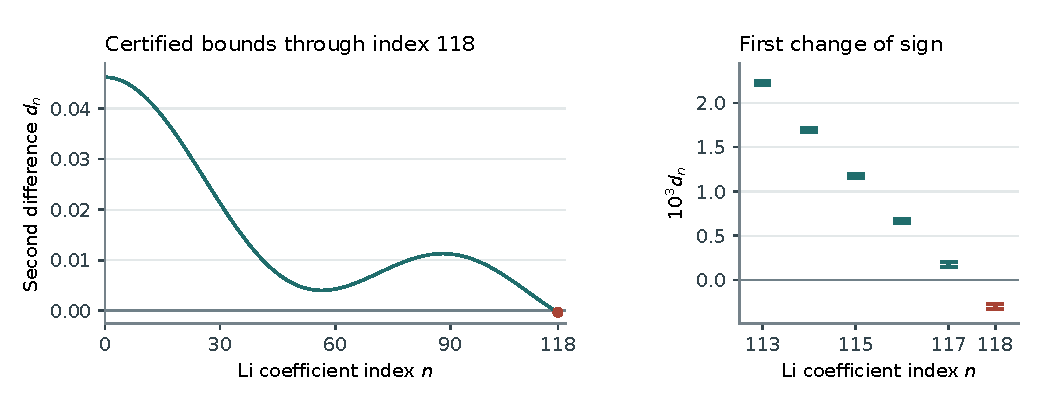
\includegraphics[width=.96\linewidth]{curvature_bounds.pdf}
\caption{Certified intervals for the centered second differences \(d_n\).
At full scale many intervals are thinner than the line. The right panel
shows the bounds on each integer separately, on an enlarged vertical scale.}
\label{fig:window}
\end{figure}

\section{Further research questions}
Can a universal test requiring weaker recurrence be proved for a class restricted by an Euler product? The finite perturbations in Corollary~\ref{cor:xi} preserve the functional equation and the high zeros, while the Euler product imposes conditions on all Dirichlet coefficients. For the actual zeta sequence, what are the limiting frequencies of the four sign regions away from their boundaries? A quantitative first-return bound for the certified signs would also give a search length for further examples.
\section{Sources and relation to earlier results}

Li proved the full-sequence criterion for Dedekind zeta functions.
Bombieri and Lagarias formulated a criterion for multisets of complex numbers
and used simultaneous phase approximation for the converse. Voros described
the exponentially oscillating contribution to the zeta coefficients when a
zero lies off the line. Lagarias developed the coefficients for automorphic
$L$-functions, including the real-part criterion used for complex characters.
These works supply the analytic setting and the mechanism by which an outer
Cayley radius affects the coefficients \cite{li,bl,voros,lag}.

The closest result in ProveIt takes dilated blocks
$\{M_j,2M_j,\ldots,jM_j\}$ for Dedekind zeta functions. It proves a positive
proportion of negative samples in each sufficiently late block if RH fails.
It also obtains the limiting normalized minimum $-m$, with $m$ the total
multiplicity on the outermost circle. The same packet uses second differences
of Li coefficients to distinguish arithmetically inequivalent fields.
Two later packets concern identification of a primitive character from
filtered fixed-stride Li samples, and simultaneous recurrence of translated
smoothed prime errors \cite{prior}.
The present classification gives a necessary and sufficient condition on an
arbitrary sampling set and realizes failure of that condition by a finite
zero multiset. For synchronized polynomial schedules the obstruction becomes
a congruence condition, with a unit constraint for prime parameters.

Bohr neighborhoods and their description by trigonometric polynomials are
classical \cite{bfw}. Weyl's theorem and Rhin's prime analogue supply the
equidistribution inputs \cite{weyl,rhin}. Bergelson, Leibman and Lesigne
proved multiple recurrence for jointly intersective polynomials.
L\^e and Spencer studied quantitative simultaneous Diophantine approximation
for intersective systems and prime analogues \cite{bll,ls}. The contribution
claimed here is the characterization for Li sums, including its converse
within the class of zero multisets. The comparison covered the 61 historical
packet READMEs and 408 TeX files in the research directories, together with
55 TeX files in 39 incoming archives at the pinned ProveIt revision.
A targeted literature search located the preceding analytic and recurrence
results. Priority for the combined theorem remains open to further comparison.

Johansson had already computed rigorous Keiper coefficients through index
100,000 \cite{joh}. For a positive index $n$, multiplying his coefficient by $n$
gives the Li normalization used here. Second differencing the published
decimals gives $d_{117}\approx0.000200147$ and
$d_{118}\approx-0.000271044$, independently confirming the initial
change of sign. Our contribution concerning this finite sign pattern is its
simultaneous recurrence at polynomially separated indices and a certificate
using forty conjugate pairs and residual moments. The computations at the
four squared indices in Table~\ref{tab:seeds} extend far beyond this table.

The survey article connects the critical-line formulation with Li
positivity \cite{wiki}. In the compact Lean edition, \texttt{src/Statements.lean}
specifies the Dirichlet zero theorem and \texttt{src/Main.lean} exports
\texttt{LFunction\_eq\_zero\_re}. The proof obtains a one-sided bound for a
weighted prime sum and passes to nonvanishing in the right half-plane.
Here its critical-line conclusion places the Cayley transforms of the
Dirichlet zeros on the unit circle. Sutherland records kernel replay and
independent checks of the exported statements for both editions \cite{lean}.
Those checks concern the upstream theorems. The sampling results above have
the mathematical proofs given in this paper.

\begin{thebibliography}{99}
\setlength{\itemsep}{2pt}
\bibitem{li} X.-J. Li, The positivity of a sequence of numbers and the
Riemann hypothesis, \emph{J. Number Theory} 65 (1997), 325--333.
\href{https://doi.org/10.1006/jnth.1997.2137}{Publisher}.
\bibitem{bl} E. Bombieri and J. C. Lagarias, Complements to Li's criterion
for the Riemann hypothesis, \emph{J. Number Theory} 77 (1999), 274--287.
\href{https://websites.umich.edu/~lagarias/doc/bombieri.pdf}{Author's copy}.
\bibitem{voros} A. Voros, Sharpenings of Li's criterion for the Riemann
hypothesis, \emph{Math. Phys. Anal. Geom.} 9 (2006), 53--63.
\href{https://doi.org/10.1007/s11040-005-9002-8}{Publisher}.
\bibitem{lag} J. C. Lagarias, Li coefficients for automorphic $L$-functions,
\emph{Ann. Inst. Fourier} 57 (2007), 1689--1740.
\href{https://doi.org/10.5802/aif.2311}{Publisher}.
\bibitem{bfw} V. Bergelson, H. Furstenberg and B. Weiss, Piecewise-Bohr sets
of integers and combinatorial number theory, Definition~1.1.
\href{https://people.math.osu.edu/bergelson.1/BFW_Bohr.pdf}{Author's copy}.
\bibitem{weyl} H. Weyl, \"Uber die Gleichverteilung von Zahlen mod. Eins,
\emph{Math. Ann.} 77 (1916), 313--352.
\href{https://doi.org/10.1007/BF01475864}{Publisher}.
\bibitem{rhin} G. Rhin, Sur la r\'epartition modulo $1$ des suites $f(p)$,
\emph{Acta Arith.} 23 (1973), 217--248.
\href{https://doi.org/10.4064/aa-23-3-217-248}{Publisher}.
\bibitem{bll} V. Bergelson, A. Leibman and E. Lesigne, Intersective
polynomials and the polynomial Szemer\'edi theorem,
\emph{Adv. Math.} 219 (2008), 369--388.
\href{https://arxiv.org/abs/0710.4862}{Preprint}.
\bibitem{ls} T. H. L\^e and C. V. Spencer, Intersective polynomials and
Diophantine approximation, \emph{Int. Math. Res. Not.} 2014 (2014), 1153--1173.
\href{https://doi.org/10.1093/imrn/rns242}{Publisher}.
\bibitem{joh} F. Johansson, Rigorous high-precision computation of the Hurwitz
zeta function and its derivatives, \emph{Numer. Algorithms} 69 (2015), 253--270.
\href{https://fredrikj.net/math/hurwitz_zeta.html}{Paper and coefficient data}.
\bibitem{prior} V. Reshetnikov, \emph{ProveIt}, Generalized Riemann Hypothesis
research collection, revision \texttt{4d7990202f9f}.
\href{https://github.com/VladimirReshetnikov/ProveIt/tree/4d7990202f9f106b2ffe8c209f073ad01d5e1987/Analysis/GeneralizedRiemannHypothesis}{Collection}.
\href{https://github.com/VladimirReshetnikov/ProveIt/blob/4d7990202f9f106b2ffe8c209f073ad01d5e1987/Analysis/GeneralizedRiemannHypothesis/Research/grh_method_transfers_research/li.tex}{Sparse dilation-block criterion}.
\href{https://github.com/VladimirReshetnikov/ProveIt/blob/4d7990202f9f106b2ffe8c209f073ad01d5e1987/Analysis/GeneralizedRiemannHypothesis/Research/grh_method_transfers_research/rigidity.tex}{Arithmetic equivalence}.
\href{https://github.com/VladimirReshetnikov/ProveIt/blob/4d7990202f9f106b2ffe8c209f073ad01d5e1987/Analysis/GeneralizedRiemannHypothesis/docs/incoming/dirichlet_li_rigidity.zip}{Filtered Li samples}.
\href{https://github.com/VladimirReshetnikov/ProveIt/blob/4d7990202f9f106b2ffe8c209f073ad01d5e1987/Analysis/GeneralizedRiemannHypothesis/docs/incoming/prime_peak_rigidity.zip}{Smoothed prime errors}.
\bibitem{lean} L. Sernau and collaborators, shorter editions of the
Alp\"oge--Claude proof of RH and GRH for Dirichlet $L$-functions,
revision \texttt{72fead102f66} (2026).
\href{https://github.com/lsernau/grh-lean/tree/72fead102f663d5c7a407964a13dc0cf9d977207}{Source}.
A. V. Sutherland, \href{https://math.mit.edu/~drew/shortgrh/}{independent verification records}.
\bibitem{wiki} Wikipedia contributors, \emph{Riemann hypothesis}, consulted
26 November 2026. \href{https://en.wikipedia.org/wiki/Riemann_hypothesis}{Article}.
\end{thebibliography}

\end{document}
